% !TeX root = ../main.tex

%TODO Andere Wege, Probleme beim IMplementieren, warum wurde etwas wie gelöst (Kleines Kind: und warum?)

\chapter{Implementation}\label{chapter:implementation}
This chapter describes details about the prototype implementation of the tool, which is written in Java.

\section{Index Creation}\label{section:implementation/index_creation}
One goal of this work is the ability to find slightly modified code.
The idea followed here is to choose the number of statements in a chunk low to react on modified, added and removed statements.
The number of statements also has to be high enough to find license infringements as defined in \autoref{section:preliminaries/infringement}.
After several tests, 5 statements per chunk seemed reasonable.

For tokenization, existing code from the work of \cite{heinemann2014teamscale} is used.
Normalization is done by iterating over all tokens and removing rather irrelevant tokens like access modifiers, brackets, the java final or the C atomic keywords.
The stream of tokens is split into statements by language dependent tokens marking the end of a statement like semicolons or curly braces in Java or C/C++.
Include or import statements are removed.
In early tests, additionally normalizing identifiers like variable names showed many false positives for variable initializations e.g. in the beginning of methods or classes.
An example for the normalization of some sample code can be found in figure \ref{fig:normalization}\todo{Finalize figure}.

\begin{figure}[h]
	\centering
	\begin{minipage}{1.2\linewidth}
		\begin{minipage}{0.35\linewidth}
			\scriptsize
			\lstinputlisting[language=C++]{data/buffer.c}
		\end{minipage}
		\begin{minipage}{0.23\linewidth}
			\scriptsize
			\begin{lstlisting}
			AVBufferRef * create uint8_t * data , ... !\tikzmark{bgnFir}!
			AVBufferRef * ref = NULL !\tikzmark{bgnSec}!
			AVBuffer * buf = NULL !\tikzmark{bgnThi}!
			buf = av_mallocz sizeof * buf
			if ! buf
			return NULL !\tikzmark{trmFir}!
			buf -> data = data !\tikzmark{trmSec}!
			buf -> size = size !\tikzmark{trmThi}!
			buf -> opaque = opaque
			atomic_init & buf -> refcount , 1
			...
			\end{lstlisting}
			
			%			\begin{tikzpicture}[overlay, remember picture]
			%			\drawBrace[.6em]{bgnFir}{trmFi}{Example xshifted.};
			%			\drawBrace{bgnSec}{trmSec}{Example annotation.};
			%			\drawBrace{bgnThi}{trmThi}{Another example.};
			%			\end{tikzpicture}
			
		\end{minipage}
	\end{minipage}
	\caption{Normalization Process}\label{fig:normalization}
\end{figure}

\todo{Problem with single statements in if/while/for without braces}
One emerging problem here are \texttt{if}, \texttt{while}, \texttt{for} or other blocks, which can be written with or without curly braces in the case of a single statement in the body.
Since the end of a statement is recognized by curly braces or semicolons as described above, a block with curly braces and a single statement is seen as multiple statements, one without the braces is seen as a single statement.
This may prevent copied code from being detected by the tool, when the braces are added or removed in the target system.
Since normalizing this case is rather complicated, it is ignored in this work.

\todo{Describe detailed storing of chunks}

A relational database can reduce the size of the store, because redundancy can be removed.
However, tests showed that even with bulk inserts, the creation of the database is more than 50 times slower than using a key-value store.
In this work RocksDB was used as a key-value store implementation.
As a hash function, MD5 is used, since it offers both, speed and high collision resistance.

As described in section \ref{section:approach/creating_index}, the key for an entry in the key-value store is the MD5 hash of a normalized chunk of code.
Since chunks with the same hash may be found in several locations, the value is a list of locations, where the chunk can be found.
For the prototypical implementation, the list for a value is serialized in JSON
Figure \ref{fig:json_serialization} shows a simplified example.

\begin{figure}[h]
	\begin{lstlisting}
		{
			[
				{
					"project": "referenceProjectName",
					"path": "src/component/ClassA.java",
					"start": 8262,
					"end": 8993,
					"revision": "ac89b33fe7a..."
				},
				{
					"project": "otherProjectName",
					"path": "src/component/SomeOtherClass.java",
					"start": 2689,
					"end": 3053,
					"revision": "893afe7b3ca..."
				},
				...
			]
		}
	\end{lstlisting}
	\caption{Simplified JSON String representing a sample value for an entry in the key-value store}\label{fig:json_serialization}
\end{figure}

\section{History Analysis}\label{section:implementation/history_analysis}
Copied code of a system may origin from a previous version of a reference system.
Modern version control systems like git, subversion or mercurial enable user to go back in time and extract any version of a source code file from the system's repository.
In this work, this is used to add old versions of source code files to the index in order to find code which has been copied from an older version of the reference system.

Versions of a repository can be seen in different granularity.
A very fine granularity would be considering every commit as a different version of the system.
On the one hand, indexing every commit would ensure that the index contains a files' content at any given point in time.
On the other hand, the number of versions and therefore the amount of files to index is huge.
Indexing large projects like that may take quite long.

First tests with a commit-based approach on the Linux kernel's master branch showed that a complete indexing would take several days to finish.
Note here that the Linux kernel code is a special case, since its git repository contains more than 600000 commits at the time of writing.
Nonetheless, this shows that commit based may be to slow for productive use.
Furthermore, changes between two commit often are minor and may not be relevant, e.g changing a constant or literal.

Instead, the implementation of this work is using a tag based approach.
First, all tags found in the reference system's repository are extracted and sorted.
After that, starting at the first tag, all files present at that point in time are indexed as described in section \ref{section:implementation/index_creation}.
Following up, for each tag in order, the changed files relative to the previous tag are indexed again.
All changed files since the last tag are re-indexed again and the key-value store is updated as described in section \ref{section:approach/creating_index/history_analysis}.

\subsection{Quick Scan}\label{section:implementation/history_analysis/quick_scan}
When a new reference project should be added to the index, no versions of the project have been scanned yet.
One way of indexing the versions defined by the available tags is to start with the tag with the oldest commit, get all files of that version and index them as described before.
After that, the next version defined by the next tag in order by date of the commit the tags are pointing to, could be indexed.

Instead of this approach indexing old to new versions of the reference project, a quicker indexing technique can be used.
The problem here is that a file often is only changed in some lines, but the bigger part of the file stays untouched.
When indexing is done from old to new, each chunk, which has not been changed, can already be found in the database pointing to the previous indexed version of the file and has to be updated.
The old entry has to be deleted and the new entry pointing to the new version of the file has to be added.
Instead, when indexing new to old versions, the entry for the chunk does not have to be changed and simply can be dropped.
This ensures that each hash in the database is pointing to the latest version of a file.

\subsection{Updating the Database}\label{section:implementation/history_analysis/update}
As explained before, the index should be updated regularly in order to find the latest copied code.
Therefore, the latest indexed version of each reference project has to be tracked.
To update the index on the server, all repositories are updated to include the latest changes.
After that, for each reference project, tags are extracted and sorted as mentioned before.
Now, instead of traversing the tags chronologically reversed, i.e from new to old tags based on the date of the commit they are pointing to, tags are scanned chronologically, i.e. from old to new.
This time, all hashes already in the database and pointing to the same file path are updated instead of dropped.

\subsection{Sorting Tags}\label{section:implementation/history_analysis/sorting_tags}
For this work, a prototype implementation for git was done.
Using git tags to get periodic snapshots of a reference system showed some difficulties during testing.

Especially for bigger projects, tags are not always sorted chronologically.
Using the tagging date may not be always accurate, since tags can be added in hindsight.
Instead, the commit date of the commit a tag is pointing to is used to sort the tags chronologically.
However, this can cause huge amounts of changed files between two tags in some cases.
One example is illustrated in \autoref{fig:tag_sort}.
For different versions, different branches exist, e.g. \texttt{v1} and \texttt{v2}.
Tags are added for every release of a version, e.g. \texttt{v1.6}.
The indexing progresses from tag to tag in chronological order by the commit date of the commit the tag is pointing to.
As the example shows, the progress is jumping between the branches causing many changed files and therefore heavily slowing down the indexing.
To compete with that, different branches of the projects where scanned as different projects.
One example is the Openjdk project, where jdk8 and jdk9 are developed on two different branches.
For each of the major versions, a copy of the project was indexed, only regarding tags, which belong to the specified version.
This could easily be done using a regular expression matching.

Another emerging problem is tags not pointing to a commit.
In git, a tag can point to any git object, such as e.g. a commit, a tree or another tag.
To deal with this circumstance, all tags not pointing to a commit where ignored during indexing.

\begin{figure}[h]
	\centering
	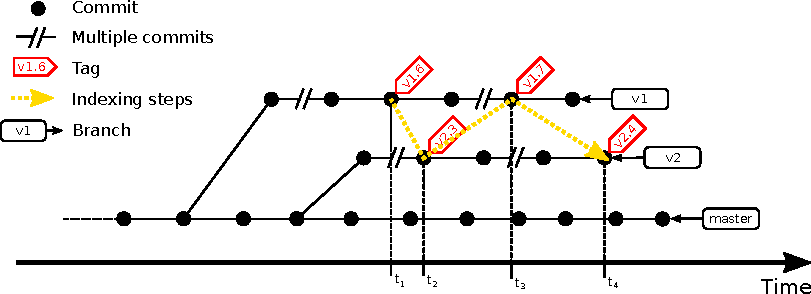
\includegraphics{figures/tag_sort.pdf}
	\caption{Tags on different branches causing many changes}\label{fig:tag_sort}
\end{figure}

Still, several problems persist: 
Clock skew amongst commiters may result in inaccurate sorting of tags and therefore could result in chunks remaining in the index not pointing to the latest version of a file.
Keeping only references to chunks of the latest version of a file seems also to be a problem when searching for copied code on a client, since matches may be scattered over multiple versions of a file, because some chunks may point to a newer version of the file instead of the version the section of code actually was copied from.
Those problems could be solved by keeping all chunks in the index, which have the same hash and are pointing to different versions of a file.
However, this would increase the size of the database drastically.
The size of the filter would not increase, since not the amount of hashes, but the amount of values a single hash is pointing to is increased.
In the prototypical implementation of the approach presented in this work, this is ignored, since scattered matches are aggregated as described in \ref{section:implementation/finding_matches}.

A better solution to sorting tags would be a branch based approach:
Every branch is followed and snapshots of the reference system are either made periodically or with the use of tags.
This may not only increase accuracy, but also indexing speed, since less files change between two versions (see \autoref{fig:tag_sort}).

\section{Hash Filter}\label{section:implementation/hash_filter}
With hash filter, this work refers to an algorithm, which can decide whether a element is part of a set with the help of a data structure which represents parts of the index.
The first approach was to simply extract the set of all hashes from the index and shorten them to reduce size, e.g. instead of 128bit per hash, only the first n bits are used.
Hashes which are equal in the first n bits but different in the remaining bits have the same shortened hash.
One hash may actually be part of the set of hashes, whereas the other may not.
With this approach a decision can not be made with absolute precision.

The probability of such a false positive can be calculated as follows:
\begin{equation}
	\frac{j}{Nenner} TODO
\end{equation}

As mentioned before, in this work a Bloom Filter is used to decide, whether a hash is contained in the index.
\todo{Bloom filter probability calculation explanation}
\todo{Compare size and probabilities: bloom filter vs shortened hashes}
\todo{Guava implementation, problems with number of hash functions}

\section{Scalability}\label{section:implementation/scalability}
The indexing process can be parallelized, which highly improves the indexing speed.
Therefore, a thread pool with 16 threads was used.
For each version of a reference project, which should be scanned, a new indexing task is created for each file of that version.
The resulting tasks are then processed by threads of the thread pool.
This is done for each version of a project and for each project, resulting on 16 threads processing one version.

Here, it is important to not change the value of a hash by different threads at the same time since this may cause a race condition.
To compete with this, a Java HashSet was used to lock the hash currently being changed by a thread.

Another difficulty is the requirement to keep the latest version of a file in the index.
To keep it simple, projects only were index one version at a time.

Tests showed, that indexing was about 8 times faster using this approach compared to a single threaded run.
The process could be parallelized even more, by concurrently indexing multiple projects at the same time.
Also it may be possible to scan multiple versions of one project at the same time, when the index keeps  references to all versions of a chunk instead only an entry pointing to the latest version of that chunk (compare section \ref{section:implementation/history_analysis/update}).
However, during test, the machine already was at its limits using this approach, leaving those options open for distributed environments.

\section{Finding Matches}\label{section:implementation/finding_matches}
For this prototypical implementation, the networking between client and server is ignored.
Instead hashes are filtered using the bloom filter and looked up by directly accessing the database containing the index.

Referring to the definitions provided in section \ref{section:preliminaries/infringement/how_much_code}, a clone is considered an infringement, if a minimum of about 8 lines of code or, in the context of this work, statements are copied.
A chunk consists of 5 statements, therefore at least two chunks have to be copied, when a single statement has been modified like illustrated in figure \ref{fig:required_chunks_modified}.
This would total in 10 copied statements, since there are no overlapping chunks.
When no statement has been modified, a sequence of statements has to consist of at least 4 chunks to contain a total of 8 statements as illustrated in figure \ref{fig:required_chunks}.
Here, 4 consecutive chunks are copied resulting in 8 copied statements without gaps.

\begin{figure}[h]
	\centering
	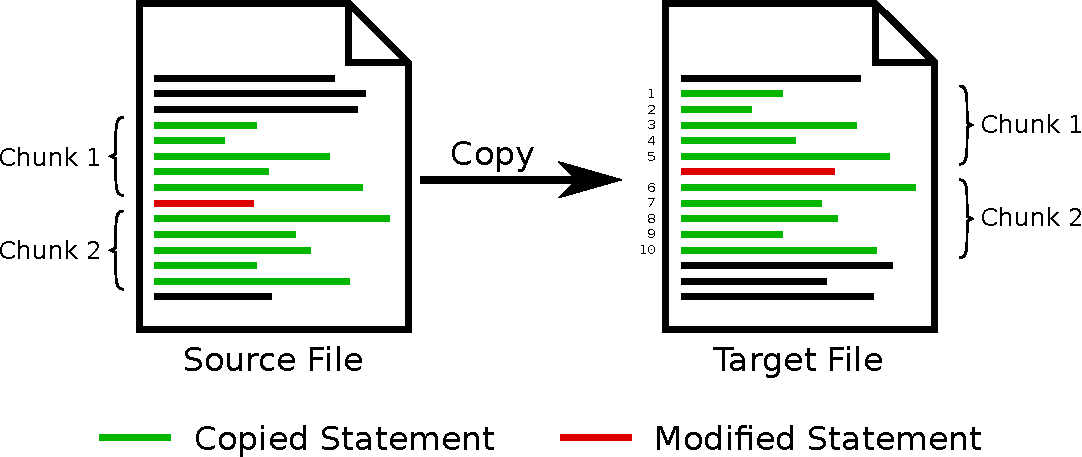
\includegraphics[width=0.9\linewidth]{figures/required_chunks_modified.pdf}
	\caption{Minimum required chunks for copied code with modification}\label{fig:required_chunks_modified}
\end{figure}

\begin{figure}[h]
	\centering
	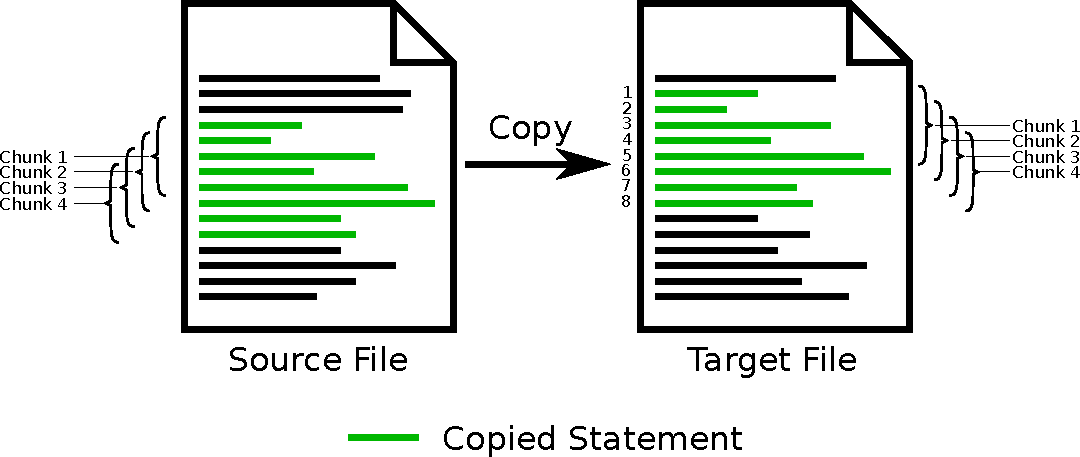
\includegraphics[width=0.9\linewidth]{figures/required_chunks.pdf}
	\caption{Minimum required chunks for copied code without modification}\label{fig:required_chunks}
\end{figure}

To compete with these limitations, for each file, chunks are extracted as described above.
The Hash Filter is used to decide whether a chunk is part of the index and therefore a match exists within the file.
If a file has less than two matching chunks, it can be ignored, since the minimum amount is two as explained above.
Otherwise, details about the matches are requested from the server by sending the list of hashes for chunks, which are marked as part of index by the filter.
The server responds with a list of locations for each hash, or an empty list, if the hash is a false positive of the Hash Filter.
\todo[inline]{describe approach for gapped clones (+4 length)}

\todo[inline]{grouping and aggregation of matches}
\todo[inline]{probability estimation: When multiple chunks of same file path (even different versions) => higher probability, when mulitple hits/match => higher probability, when many different files, only small amount of hits/match = low probability}
\todo[inline]{Describe possibilities for continuous detection}
